% Indicate the main file. Must go at the beginning of the file.
% !TEX root = ../main.tex

%----------------------------------------------------------------------------------------
% CHAPTER 4
%----------------------------------------------------------------------------------------
\chapter{Methodology} % Main chapter title
\label{Chapter4} % For referencing the chapter elsewhere, use \ref{Chapter1}

\section{Data}

The data was provided by [Eawag, institute of Aquatic Sciences]. It was generated using CADDIE2D software, which is described in Chapter \ref{Chapter3}. In the dataset, we look at four catchment areas around Switzerland, '26', '292', '709', '819' (see Fig \ref{fig:4.1}). They are named according to a DEM naming scheme all DEM's have a spatial resolution of 1. For each DEM, there are fourteen rainfall events (see \ref{fig:4.2}). For each rainfall event, there is a water depth  map for each time step (see Fig \ref{fig:4.3}, which shows spatial evolution over time). The dataset provided also contains rainfall event names and  finally, a mask to remove areas outside the catchment area (if water were to propagate to this boundary, it would be considered run-off). Each time step represents 10 minutes of real time, but computational time of the CADDIES model varies for each time step computed.

\begin{figure}[htbp]
	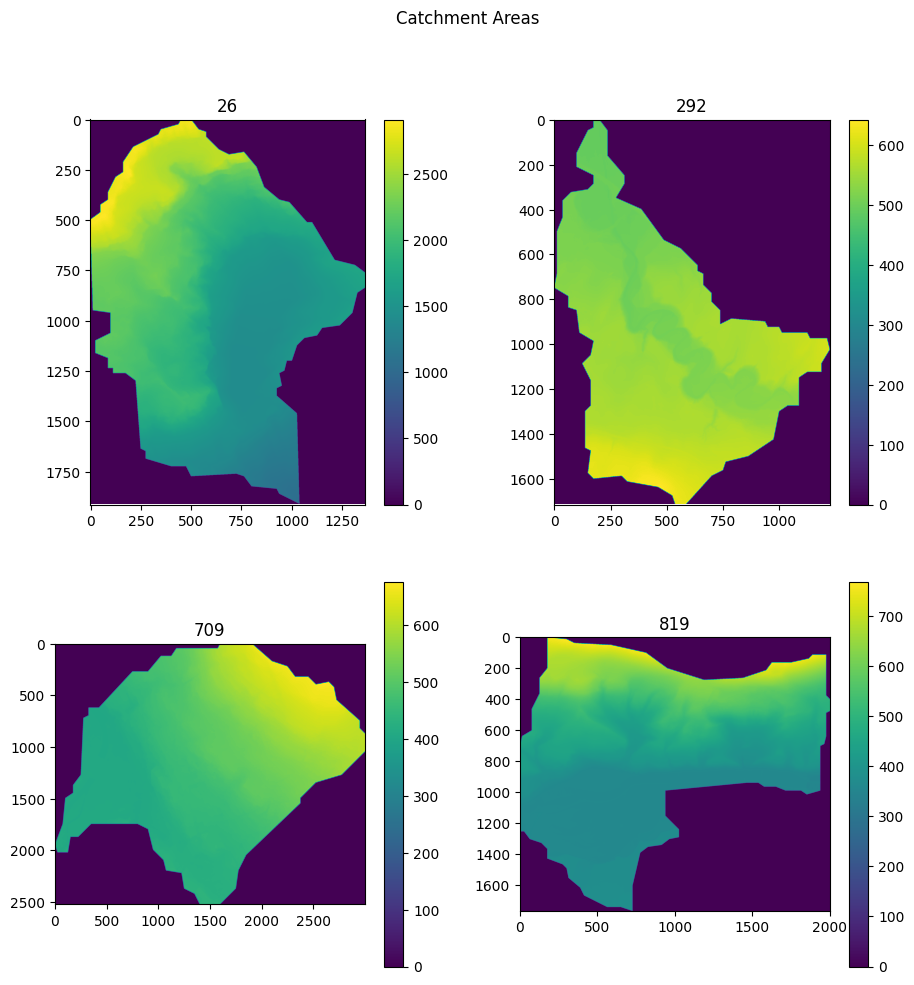
\includegraphics[width=0.6\textwidth]{../Figures/Catchment_dems.png}
	\centering
	\caption[FourDems]{Elevation map for the four catchment areas of interest. Color indicates height in m; height of 0 m is outside of the catchment area} 
	\label{fig:4.1}
\end{figure}

\begin{figure}[htbp]
	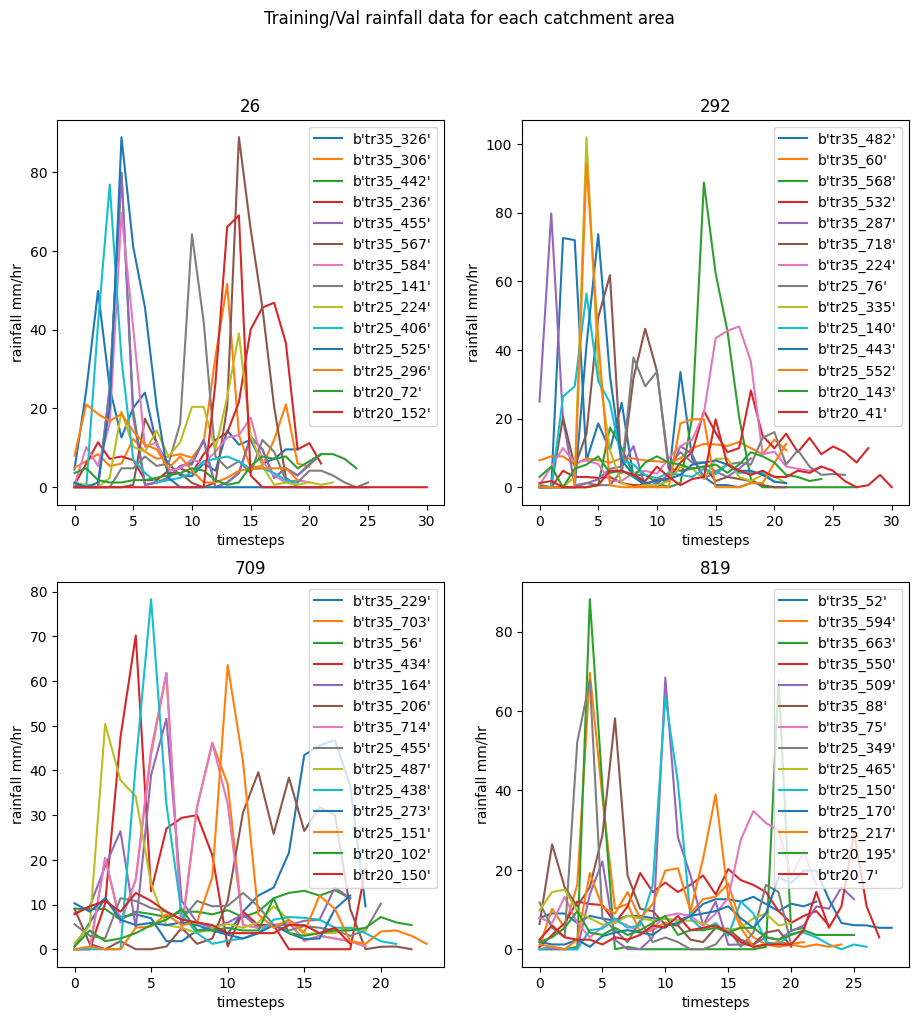
\includegraphics[width=0.6\textwidth]{../Figures/rainfall_train.png}
	\centering
	\caption[rainfall events]{Rainfall events over time for each DEM} 
	\label{fig:4.2}
\end{figure}

\begin{figure}[htbp]
	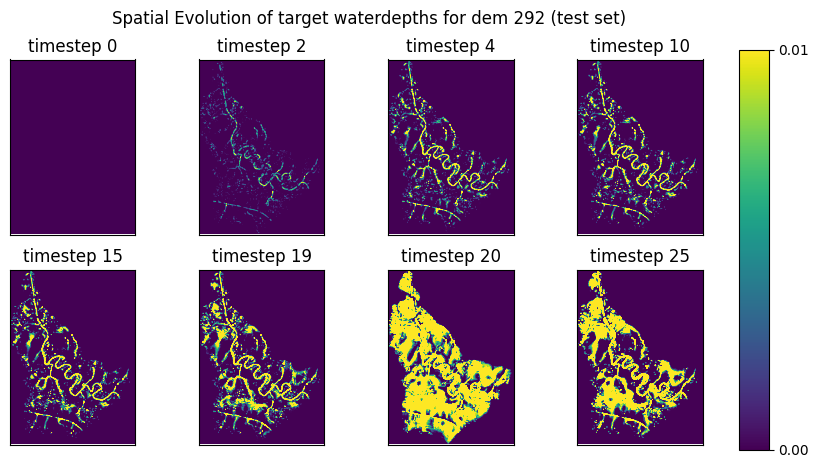
\includegraphics[width=0.6\textwidth]{../Figures/spatial_evoltution_waterdepth.png}
	\centering
	\caption[wd spatial evolution]{Spatial evolution of water depths for catchment 292. Colour indicates waterdepth (in m)} 
	\label{fig:4.3}
\end{figure}


\subsection{Data Preprocessing}
Due to computational limitations, data used during training are sub-sampled to have spatial dimensions 120 x 120, while the data used for testing has spatial dimensions 400 x 400 The rainfall events, titled "rainfall \_ events \_ 0 - 13", are used for training and validation data (using the train \_ test \_ split function from the sklearn library) in a ratio of 0.8 and 0.2 respectively. The last  rainfall  event "rainfall \_ events \_ 14" is unseen and used for the test set (see Fig \ref{fig:4.4}). \\
Many datasets were created but what has been mentioned above is consistent for all of them.

\begin{figure}[htbp]
	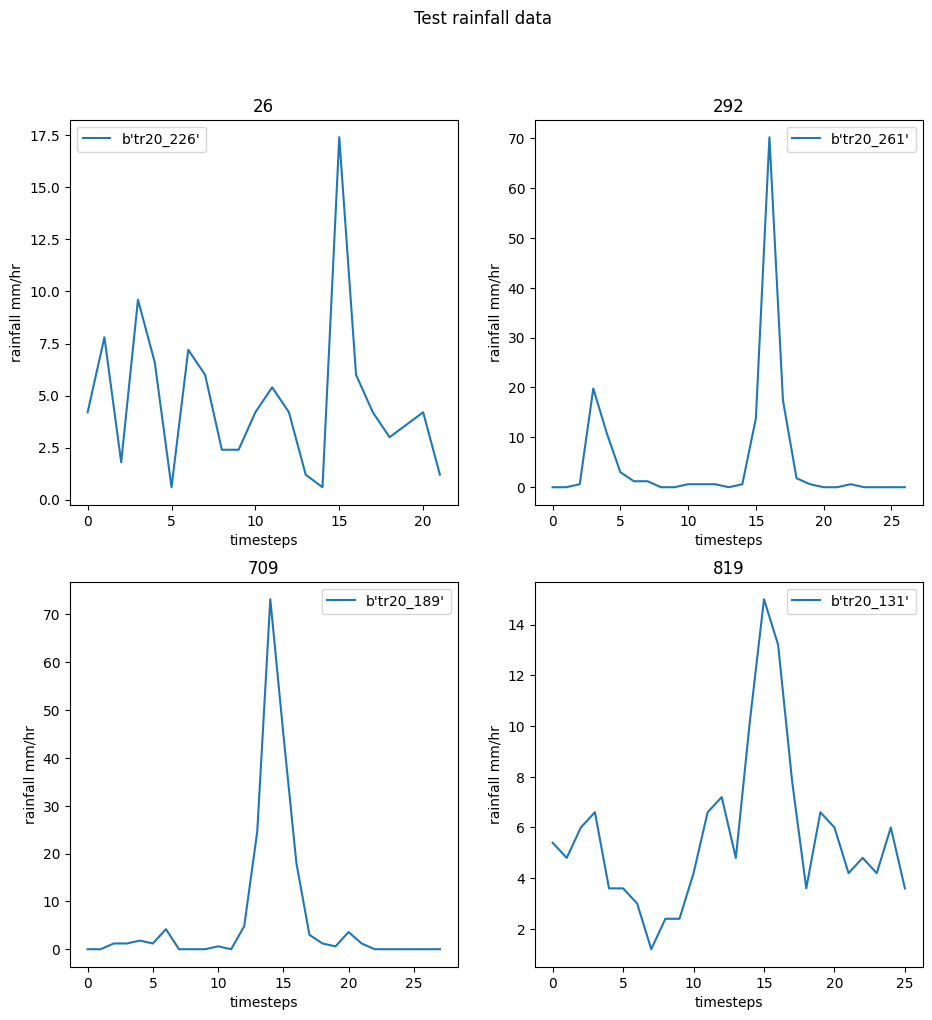
\includegraphics[width=0.6\textwidth]{../Figures/test_rainfall_events.png}
	\centering
	\caption[Rainfall Test]{Rainfall events used for testing} 
	\label{fig:4.4}
\end{figure}

\subsubsection*{Initial Screening}
\label{methods:inital-screening}
Three datasets were created for each DEM. All datasets use the same features:
\begin{enumerate}
	\item Water depth (meters)
	\item Rainfall (mm/hr)
	\item DEM
\end{enumerate}

A representation of the tensor can be seen in Figure \ref{fig:4.5} \\

\begin{figure}[htbp]
	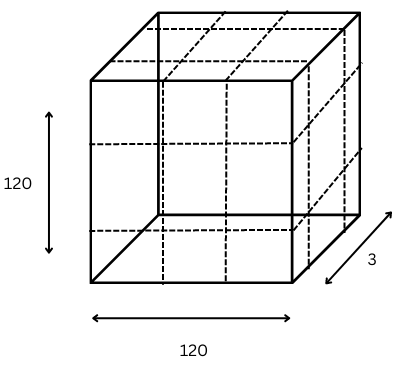
\includegraphics[width=0.5\textwidth]{../Figures/dataset_visualization}
	\centering
	\caption[training data]{The shape of training data. Made using Canvas}
	\url{https://www.canva.com/}
	\label{fig:4.5}
\end{figure}

The first dataset uses the raw features generated by the CADDIES model. The second dataset uses Min Max normalization but across all features by normalizing via the DEM (see Eq. \ref{eq:4.1}). The third uses classical min max normalization (see Eq. \ref{eq:4.2}) for the DEM feature, rainfall is interpolated over time (see Eq \ref{eq:4.3}), and the water depth is just divided by a constant  (see Eq \ref{eq:4.4}).

\begin{equation}
	\label{eq:4.1}
	X_{norm} = \frac{X-A_{min}}{A_{max}-A_{min}}
\end{equation}

\begin{equation}
	\label{eq:4.2}
	X_{norm} = \frac{X-X_{min}}{X_{max}-X_{min}}
\end{equation}
Where $X$ is the feature to be normalized, $A$ is the whole dataset.
\begin{equation}
	\label{eq:4.3}
	r_{interpolated} = \frac{\frac{r}{1000}}{60} \times 10
\end{equation}
Where $r$ is rainfall in mm/hr. The interpolated rainfall is in m/ 10 minutes.
\begin{equation}
	\label{eq:4.4}
	X_{w \_ normed} = \frac{X_{w}}{8}  
\end{equation}

Where $X_{w}$ is the water depth feature. The reason to divide by 8 is to drive the water depths to a range between 0 and 1 without making the values too small. As there was a lot of variation of water depths.

\subsubsection*{Additional Features}
Two additional datasets were created for evaluation. The first Adds the DEM mask to the feature list. The motivation for this is to guarantee  runoff occurs outside the catchment areas. The second dataset adds rainfall directly to the water depth and we are left with only two features.

\section{Models}

\subsubsection*{Initial Screening}
\label{DepthwiseCNN:init}
From previous evaluation, A simple depth-wise CNN seemed to work well.  So the following model (see \ref{lst:1}) was used for evaluation on the initial screening dataset:

\begin{lstlisting}[language=Python, label={lst:1}]
	class DepthwiseCNN(tf.keras.Model):
	def __init__(self):
		super().__init__()
		self.dmodel = tf.keras.Sequential([
		tf.keras.layers.Conv2D(8, 1, activation=tf.nn.relu, padding="same"),
		tf.keras.layers.DepthwiseConv2D(3, depth_multiplier = 10, activation=tf.nn.relu, padding="same"),
		tf.keras.layers.Conv2D(8, 1, activation=tf.nn.relu, padding="same"),
		tf.keras.layers.Conv2D(1, 1, activation=None, padding="same", kernel_initializer=tf.zeros_initializer)
		])
		self(tf.zeros([1, 3, 3, 3]))
	
	
	def call(self, x):
		dx = self.dmodel(x) # Predict the difference
		f1, f2, f3 = tf.unstack(x, axis=-1) #  f1 is wd
		f1 =tf.expand_dims(f1, -1)
		return dx + f1 # return summed wd
	
\end{lstlisting}
The initial screening model has the following model summary,

\begin{verbatim}
	Model: "Inital Screening"
	_________________________________________________________________
	Layer (type)                 Output Shape              Param #   
	=================================================================
	sequential (Sequential)      (1, 3, 3, 1)              1489      
	=================================================================
	Total params: 1,489
	Trainable params: 1,489
	Non-trainable params: 0
	_________________________________________________________________
	None
\end{verbatim}

\subsubsection*{Adding Complexity}
Here a grid search is done using configuration files (see listing \ref{lst:3} for an example configuration) on a modified model based on listing \ref{lst:1}. See listing \ref{lst:2}.
\begin{lstlisting}[language=Python,  label={lst:2}]

class DepthwiseCNN(tf.keras.Model):
	def __init__(self, model_config, dset_config):
		super().__init__()
		self.dset_config = dset_config
		self.model_config = model_config
		self.dmodel = tf.keras.Sequential([
		tf.keras.layers.Conv2D(self.model_config['first1x1'], 2, activation=tf.nn.relu, padding="same"),
		tf.keras.layers.DepthwiseConv2D(3, activation=tf.nn.relu, padding="same", depth_multiplier=self.model_config['depth']),
		tf.keras.layers.Conv2D(self.model_config['second1x1'], 1, activation=tf.nn.relu, padding="same"),
		tf.keras.layers.Conv2D(1, 1, activation=None, padding="same", kernel_initializer=tf.zeros_initializer)
		])
		self(tf.zeros([1, 3, 3, self.dset_config['num_features']]))

	def call(self, x):
	
		if self.model_config['diff']:
			dx = self.dmodel(x)
			
			if self.dset_config['mask']:
				f1, f2, f3, f4 = tf.unstack(x, axis=-1)
				f1 = tf.expand_dims(f1, -1)
				return dx + f1
		
			elif self.dset_config['added_rainfall']:
				f1, f2, = tf.unstack(x, axis=-1)
				f1 = tf.expand_dims(f1, -1)
				return dx + f1
			else:
				f1, f2, f3 = tf.unstack(x, axis=-1)
				f1 = tf.expand_dims(f1, -1)
				return dx + f1
		
		else:
			dx = self.dmodel(x)
			return dx
	
\end{lstlisting}

\begin{lstlisting}[language=Python, label={lst:3}]

	model_config2 = {
		'name': 'medium_depthwise_diff',
		'depth': 8,
		'first1x1': 8,
		'second1x1': 16,
		'n_features': 3,
		'diff': True
	}

\end{lstlisting}

Three models are looked at. Shallow, Medium, and Complex models. Their model summaries, respectively, are,

\begin{verbatim}
	Model: "depthwise_shallow"
	_________________________________________________________________
	Layer (type)                 Output Shape              Param #   
	=================================================================
	sequential_2 (Sequential)    (1, 3, 3, 1)              265       
	=================================================================
	Total params: 265
	Trainable params: 265
	Non-trainable params: 0
	_________________________________________________________________
	None
\end{verbatim}

\begin{verbatim}
	Model: "depthwise_medium"
	_________________________________________________________________
	Layer (type)                 Output Shape              Param #   
	=================================================================
	sequential_3 (Sequential)    (1, 3, 3, 1)              1801      
	=================================================================
	Total params: 1,801
	Trainable params: 1,801
	Non-trainable params: 0
	_________________________________________________________________
	None
\end{verbatim}

\begin{verbatim}
	Model: "depthwise_complex"
	_________________________________________________________________
	Layer (type)                 Output Shape              Param #   
	=================================================================
	sequential_4 (Sequential)    (1, 3, 3, 1)              23913     
	=================================================================
	Total params: 23,913
	Trainable params: 23,913
	Non-trainable params: 0
	_________________________________________________________________
	None
\end{verbatim}

\subsubsection*{Inception Block Inspired}
The last model looked at was an Inception Block Inspired model with  varying complexity (see Listing \ref{lst:4}) with an example configuration (see Listing \ref{lst:5}). The use of this architecture is motivated by the fact that very few features are used as input and the inception block architecture is enrich the feature space through the use of sub networks \cite{ding2021diverse}

\begin{lstlisting}[language=Python, label={lst:4}]
	
class IncepInspired(tf.keras.Model):
	def __init__(self, model_config, dset_config):
		super().__init__()
		self.dset_config = dset_config
		self.model_config = model_config
		self.depth = tf.keras.Sequential([
		tf.keras.layers.DepthwiseConv2D(5, activation=tf.nn.relu, padding="same", depth_multiplier=self.model_config['depth']),
		tf.keras.layers.Conv2D(self.model_config['depth_1x1'], 1, activation=tf.nn.relu, padding="same")
		])
		self.conv = tf.keras.Sequential([
		tf.keras.layers.Conv2D(self.model_config['conv_filter_1'],5 , activation=tf.nn.relu, padding="same"),
		tf.keras.layers.Conv2D(self.model_config['conv_filter_2'], 5, activation=tf.nn.relu, padding="same"),
		])
		
		self.conv1x1 = tf.keras.Sequential([
		tf.keras.layers.Conv2D(self.model_config['conv_1x1'] ,1, activation=tf.nn.relu, padding="same"),
		])
		
		self.dmodel = tf.keras.Sequential([
		tf.keras.layers.Conv2D(self.model_config['first_3x3'], 5, activation=tf.nn.relu, padding="same"),
		tf.keras.layers.Conv2D(self.model_config['first1x1'], 1, activation=tf.nn.relu, padding="same"),
		tf.keras.layers.Conv2D(self.model_config['second1x1'], 1, activation=tf.nn.relu, padding="same"),
		tf.keras.layers.Conv2D(1, 1, activation=None, padding="same", kernel_initializer=tf.zeros_initializer)
		])
		self(tf.zeros([1, 3, 3, self.dset_config['num_features']]))
	
	def call(self, x):
	
		if self.model_config['diff']:
			x1 = self.depth(x)
			x2 = self.conv(x)
			x3 = self.conv1x1(x)
			y = tf.concat([x1,x2,x3], axis=-1)
			
			dx = self.dmodel(y)
			
			if self.dset_config['mask']:
				f1, f2, f3, f4 = tf.unstack(x, axis=-1)
				f1 = tf.expand_dims(f1, -1)
				return dx + f1
			
			elif self.dset_config['added_rainfall']:
				f1, f2, = tf.unstack(x, axis=-1)
				f1 = tf.expand_dims(f1, -1)
				return dx + f1
			else:
				f1, f2, f3 = tf.unstack(x, axis=-1)
				f1 = tf.expand_dims(f1, -1)
				return dx + f1
		
		else:
			x1 = self.depth(x)
			x2 = self.conv(x)
			x3 = self.conv1x1(x)
			y = tf.stack([x1,x2,x3], axis=-1)
			dx = self.dmodel(y)
			return dx
	
\end{lstlisting}

\begin{lstlisting}[language=Python, label={lst:5}]
	incep_config2 = {
		'name': 'medium_incep',
		'depth': 8,
		'depth_1x1': 12,
		'conv_filter_1': 32,
		'conv_filter_2': 12,
		'conv_1x1': 12,
		'first_3x3': 32,
		'first1x1': 8,
		'second1x1': 16,
		'diff': True,
		
	}
	
\end{lstlisting}
Two versions of the model are created: Simple and Medium \footnote{The complex model was not able to train properly on the authors computer}.
They have the following model summaries,

\begin{verbatim}
	Model: "incep_inspired_simple"
	_________________________________________________________________
	Layer (type)                 Output Shape              Param #   
	=================================================================
	sequential_5 (Sequential)    (1, 3, 3, 8)              110       
	_________________________________________________________________
	sequential_6 (Sequential)    (1, 3, 3, 8)              1388      
	_________________________________________________________________
	sequential_7 (Sequential)    (1, 3, 3, 8)              32        
	_________________________________________________________________
	sequential_8 (Sequential)    (1, 3, 3, 1)              5041      
	=================================================================
	Total params: 6,571
	Trainable params: 6,571
	Non-trainable params: 0
	_________________________________________________________________
	None
\end{verbatim}

\begin{verbatim}
	Model: "incep_inspired_medium"
	_________________________________________________________________
	Layer (type)                 Output Shape              Param #   
	=================================================================
	sequential_9 (Sequential)    (1, 3, 3, 12)             924       
	_________________________________________________________________
	sequential_10 (Sequential)   (1, 3, 3, 12)             12044     
	_________________________________________________________________
	sequential_11 (Sequential)   (1, 3, 3, 12)             48        
	_________________________________________________________________
	sequential_12 (Sequential)   (1, 3, 3, 1)              29257     
	=================================================================
	Total params: 42,273
	Trainable params: 42,273
	Non-trainable params: 0
	_________________________________________________________________
	None
\end{verbatim}


\section{Training}
\subsubsection*{Loss Functions}
\label{training:loss}
MSE (see Eq. \ref{eq:2.2}) and MAE (see Eq. \ref{eq:2.3}) were evaluated as well as two variations of regularization (see Eq. \ref{eq:4.5} and Eq. \ref{eq:4.6}) for each for a total of six loss functions.
\begin{equation}
	\label{eq:4.5}
	 R_{auto} = (W_{z} + W_{nz})
\end{equation}
Where $W{z}$ is the zero weight matrix calculated by summing the zeros in $\hat{y}_{i}$ and divided by the total number of elements. $W_{nz}$ is the non-zero weight matrix calculated by summing the non zero elements and dividing by the total number of elements. $R_{auto}$ was named such because it automatically adjusts the weighting based on current sub section of data.
\begin{equation}
	\label{eq:4.6}
	R_{manual} = (W_{z} + W_{nz})
\end{equation}
Where $W{z}$ is the zero weight that is a chosen parameter. $W_{nz}$ is the non zero weight that is a chosen parameter. $R_{manual}$ is the Regularization term.

The loss functions now become,
\begin{equation}
	\label{4.7}
	Loss = (error \cdot R) \frac{1}{n}
\end{equation}
where $error$ is either Sum of Square Error or Absolute Error. $R$ is either of the regularization terms in Eq. \ref{eq:4.5} or Eq. \ref{eq:4.6}.

\subsubsection*{Hyper Parameter Tuning}
In previous evaluation, the Adam optimizer performed the best and so was used for training in this thesis. A consistent batch size is across training. It was found to be a happy medium between amount of samples in each batch and computer memory. The learning rate for the Adam optimizer as well as number of Epochs (number of iterations through the whole dataset) was determined using a grid search method. \\

Along with the above, models were evaluated on predicting water difference versus predicting the water depth directly.

\section{Evaluation}

\subsubsection*{Baseline Models}
Two shallow deep learning models are used for comparison. The first is a slightly shallower version of the Fully Convolutional Network used by \citeauthor{russo2023evaluation}.

\begin{lstlisting}[language=Python, label={lst:6}]
class BenchMark1(tf.keras.Model): # Benchmark from the evalution paper (but reduced, do to computational constraints)
	def __init__(self, model_config, dset_config):
		super().__init__()
		self.dset_config = dset_config
		self.model_config = model_config
		self.dmodel = tf.keras.Sequential([
		tf.keras.layers.Conv2D(16, 5, padding="same", activation=tf.nn.relu),
		tf.keras.layers.Conv2D(32, 5, padding="same", activation=tf.nn.relu),
		tf.keras.layers.Conv2D(32, 5, padding="same", activation=tf.nn.relu),
		tf.keras.layers.Conv2D(1, 1, activation=None)
		])
		self(tf.zeros([1, 3, 3, self.dset_config['num_features']]))

	def call(self, x):
	
		if self.model_config['diff']:
			dx = self.dmodel(x)
			
			if self.dset_config['mask']:
				f1, f2, f3, f4 = tf.unstack(x, axis=-1)
				f1 = tf.expand_dims(f1, -1)
				return dx + f1
			
			elif self.dset_config['added_rainfall']:
				f1, f2, = tf.unstack(x, axis=-1)
				f1 = tf.expand_dims(f1, -1)
				return dx + f1
			else:
				f1, f2, f3 = tf.unstack(x, axis=-1)
				f1 = tf.expand_dims(f1, -1)
				return dx + f1
		
		else:
			dx = self.dmodel(x)
			return dx
	
\end{lstlisting}
The above baseline model has a model summary,
\begin{verbatim}
	Model: "bench_mark1"
	_________________________________________________________________
	Layer (type)                 Output Shape              Param #   
	=================================================================
	sequential (Sequential)      (1, 3, 3, 1)              39713     
	=================================================================
	Total params: 39,713
	Trainable params: 39,713
	Non-trainable params: 0
	_________________________________________________________________
	None
\end{verbatim}

The second benchmark model is a simple CNN but characterized by 1x1 convolutions in the second and third layer of the model. This model was established in prior testing.

\begin{lstlisting}[language=Python, label={lst:7}]
	class BenchMark2(tf.keras.Model): # simple model characterized by 1x1 convolutions
		def __init__(self, model_config, dset_config):
			super().__init__()
			self.model_config = model_config
			self.dset_config = dset_config
			self.dmodel = tf.keras.Sequential([
			tf.keras.layers.Conv2D(80, 3, padding="same", activation=tf.nn.relu),
			tf.keras.layers.Conv2D(64, 1, activation=tf.nn.relu),
			tf.keras.layers.Conv2D(1, 1, activation=None)
			])
			self(tf.zeros([1, 3, 3, self.dset_config['num_features']]))
		
		def call(self, x):
		
			if self.model_config['diff']:
				dx = self.dmodel(x)
				
				if self.dset_config['mask']:
					f1, f2, f3, f4 = tf.unstack(x, axis=-1)
					f1 = tf.expand_dims(f1, -1)
					return dx + f1
				
				elif self.dset_config['added_rainfall']:
					f1, f2, = tf.unstack(x, axis=-1)
					f1 = tf.expand_dims(f1, -1)
					return dx + f1
				else:
					f1, f2, f3 = tf.unstack(x, axis=-1)
					f1 = tf.expand_dims(f1, -1)
					return dx + f1
			
			else:
				dx = self.dmodel(x)
				return dx
\end{lstlisting}

It has a model summary of,
\begin{verbatim}
	Model: "bench_mark2"
	_________________________________________________________________
	Layer (type)                 Output Shape              Param #   
	=================================================================
	sequential_1 (Sequential)    (1, 3, 3, 1)              7489      
	=================================================================
	Total params: 7,489
	Trainable params: 7,489
	Non-trainable params: 0
	_________________________________________________________________
	None
\end{verbatim}


And finally a simple heuristic is used for a complete comparison. The heuristic is predicting the previous time step with no change (see Eq. \ref{eq:4.7}) \footnote{The roll function from the numpy module in python was used as the heuristic. An oversight occured and instead of evaluating on no change (the original idea), the heuristic instead predicts the previous time step. What was meant to be evaluated was $X_{w}^{t+1} = X_{w}^{t}$}. Evaluation is done on all the baseline models for predicting a single time step ahead (10 minutes). But a recurrent version is also tested. After training the models, The output of the model becomes the new input. This is done for all time steps in the test data set.

\begin{equation}
	\label{eq:4.7}
	X_{w}^{t+1} =  X_{w}^{t-1}
\end{equation}
Where $X_{w}^{t}$ is the water depth at time $t$.

\subsubsection*{Metric}
The proposed metric for evaluating the model is to use MAE (see Eq. \ref{eq:2.3}). The goal is to minimize this as much as possible and to perform better than the baseline models and heuristic.